\begin{section}{Power Spectra and Information Content}
  \label{sec:fisherinfo}
    The power spectrum is the Fourier transform of the correlation function and measures
 the amoutn of clustering in the matter distribution in terms of the wavenumber
 $k$ in unit of $h \mathrm{Mpc}^{-1}$,
\begin{align}
    \langle \delta \left( \bm{k} \right) \delta \left( \bm{k'}\right) \rangle =
\left( 2\pi \right) ^3 P \left( \bm{k} \right) \hat{\delta} \left( \bm{k}-\bm{k'} \right),
\end{align}
where $\delta \left( \bm{k} \right)$ is the density fluctuation in wave space, while 
$\hat{\delta}$ is the delta funciton. Of equal interest is $\Delta ^2_k$, the power 
spectrum in its dimensionless form, defined as
\begin{align}
    \Delta ^2_k \equiv \frac{k^3 P \left( k \right)}{2\pi ^2}
\end{align}
    The power spectra of the mass distributions are calculated using the "Nearest Grid Point" 
(NGP) mass assignment scheme, which calculates the position of each particle based on which 
grid point it is nearest. In Fig.\ref{fig:powerspectrum} we plot the mean power spectrum (and 
error bars) of 136 linear and non-linear density fields and reconstruced density fields simply 
given by $\delta_r=\bm{k}\bm{k}\xi$, and their cross correlation with linear density fields. 
The linear density field is given by the linear density field at $z=0$.
\begin{figure}[t!]
\begin{center}
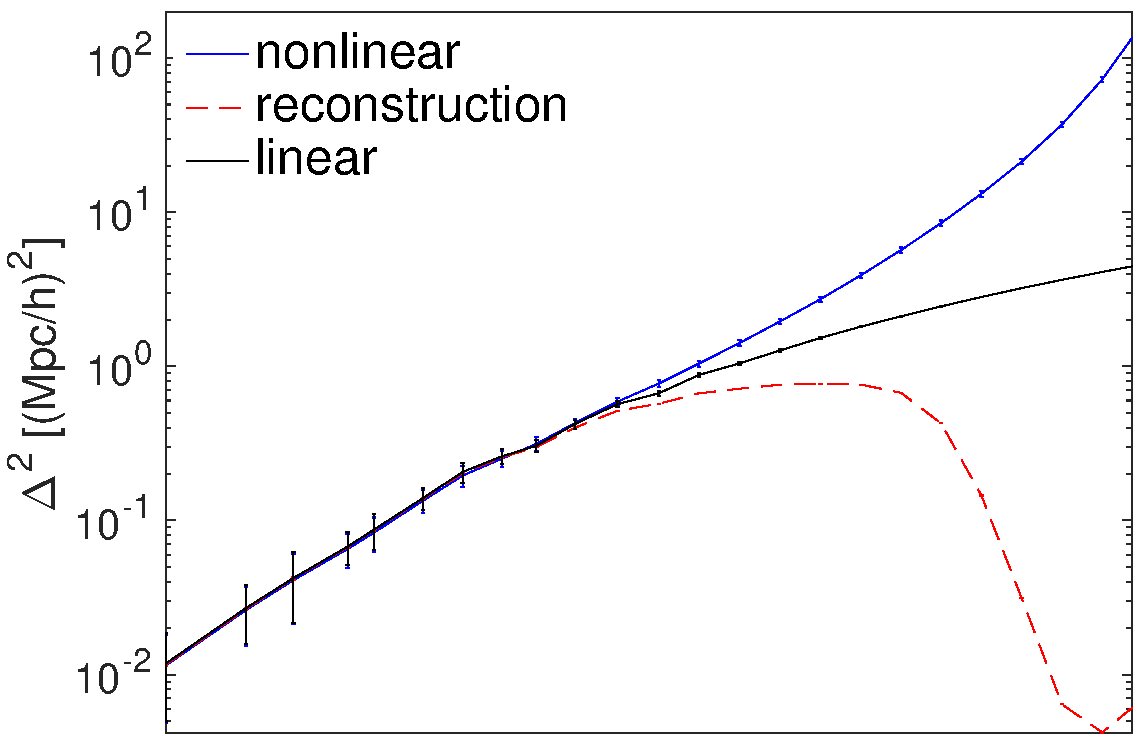
\includegraphics[width=0.48\textwidth]{powerspectrum_good-crop.pdf}
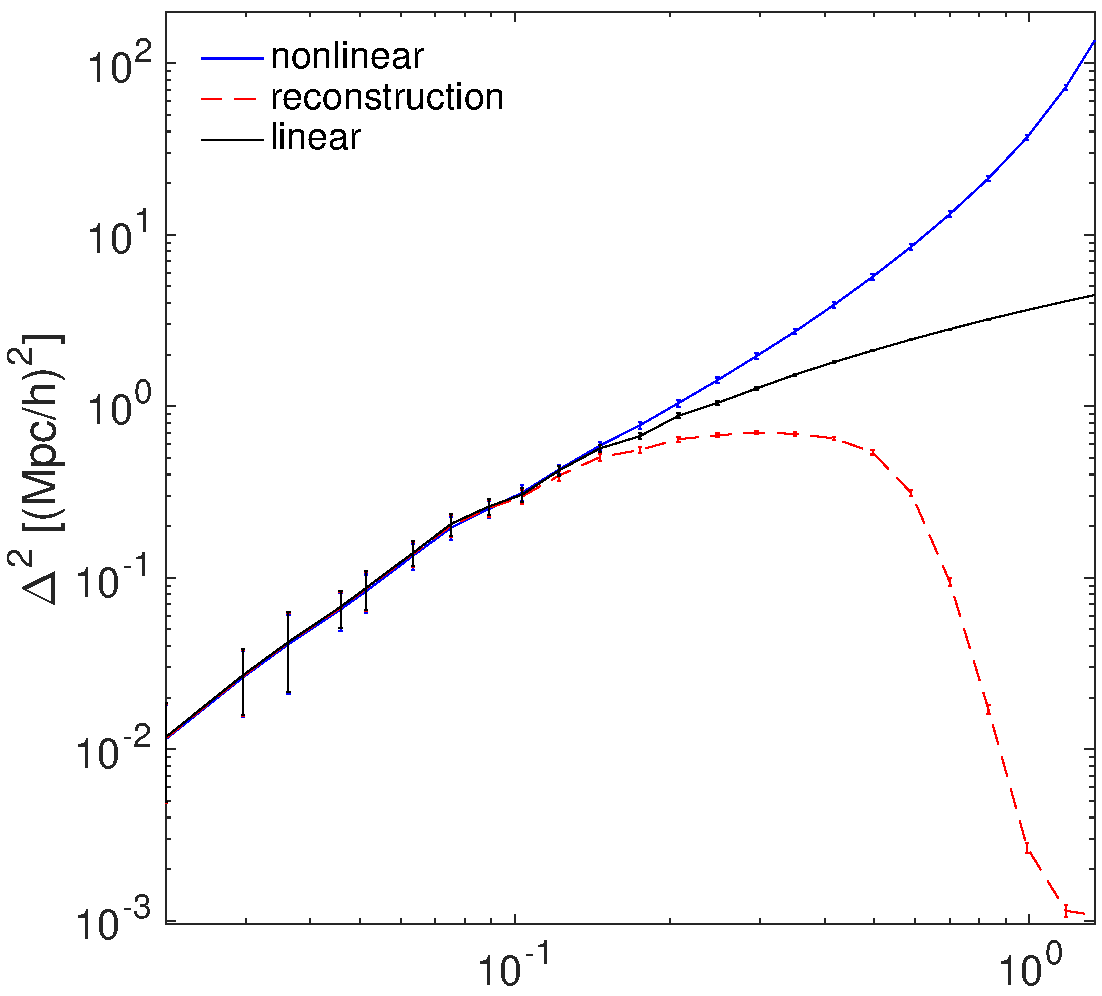
\includegraphics[width=0.48\textwidth]{power_rectolin-crop.pdf}
\end{center}
\begin{flushright}
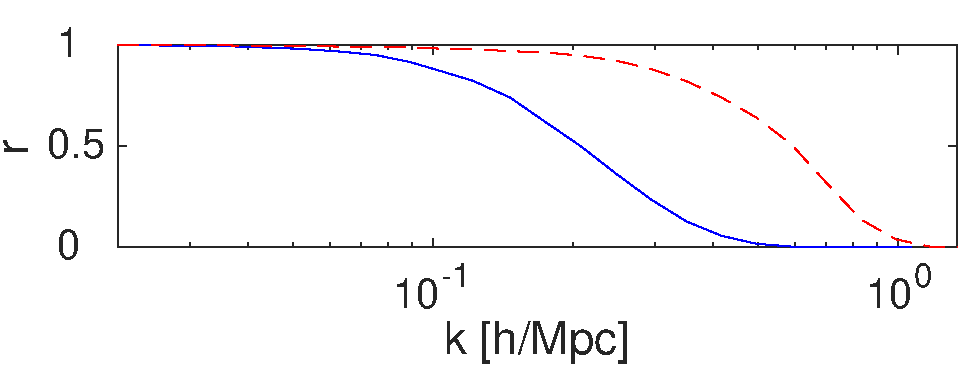
\includegraphics[width=0.48\textwidth,height=0.1\textwidth]{correlation_good-crop.pdf}
\end{flushright}
\caption{(Upper)Mean power spectrum with error bar of 136 linear density fields, non-linear 
density fields and reconstruced density fields.(Lower)Mean cross correlation of non-linear 
density fields and reconstructed density fields with linear density fields.}
\end{figure}

%    To calculate the cumulative Fisher information of the density fields, the covariance matrix 
%of the power spectra should be first given. Mathematically, the the covariance matrix is defined as
%\begin{align}
%    \mathrm{Cov}\left(k,k'\right)\equiv \frac{1}{N-1}\sum_{i=1}^{N}\left[ P_i \left( k \right) - 
%\langle P \left( k \right) \rangle \right]\left[ P_j \left( k' \right) - \langle P \left( k' \right)\rangle \right],
%\end{align}
%where angle brackets mean the expected values. 
%    The the correlation matrix, is a 
%normalized version of the covariance matrix,
%\begin{align}
%    \mathrm{Corr}\left(k,k'\right)=\frac{\mathrm{Cov}\left(k,k'\right)}{\sqrt{\mathrm{Cov}\left(k,k\right)\mathrm{Cov}\left(k',k'\right)}}.
%\end{align}
%The corelation matrices for density fields from simulations and deformation potentials from 
%reconstructions are shown in Fig. \ref{fig:corrall}. For the original density fields, the 
%linear regime, where $k<0.1$, is diagonal, while in the non-linear regime, the power spectra of 
%different $k$ modes are strongly correlated by at least $60\%$ . For the reconstructed deformation 
%potential correlation matrix, however, the linear regime expand up to $k~0.2$. The correlation 
%matrix is closer to that for the power spectra of linear density fields.
%\begin{figure}
% \centering
%  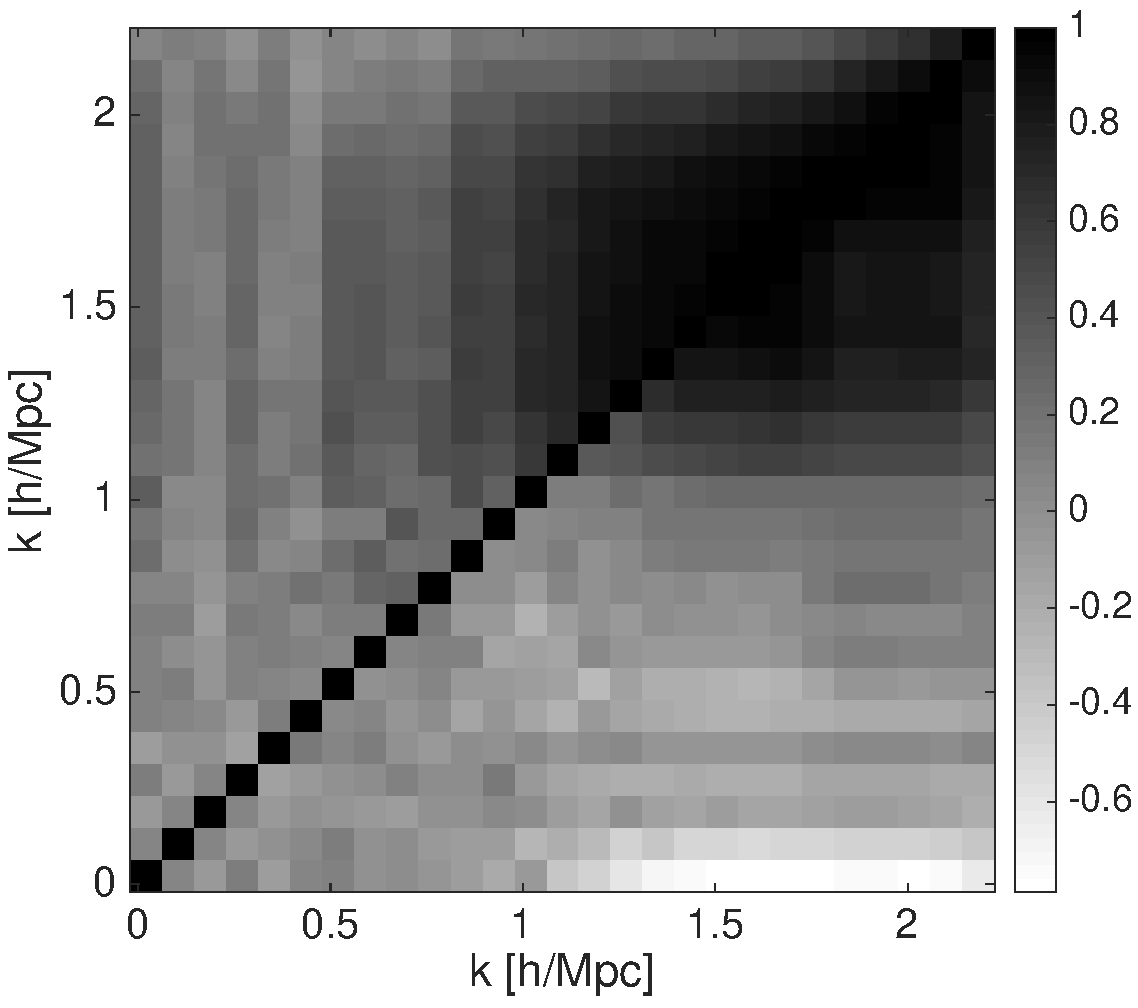
\includegraphics[width=0.48\textwidth]{corrmatrix_good-crop.pdf}
%  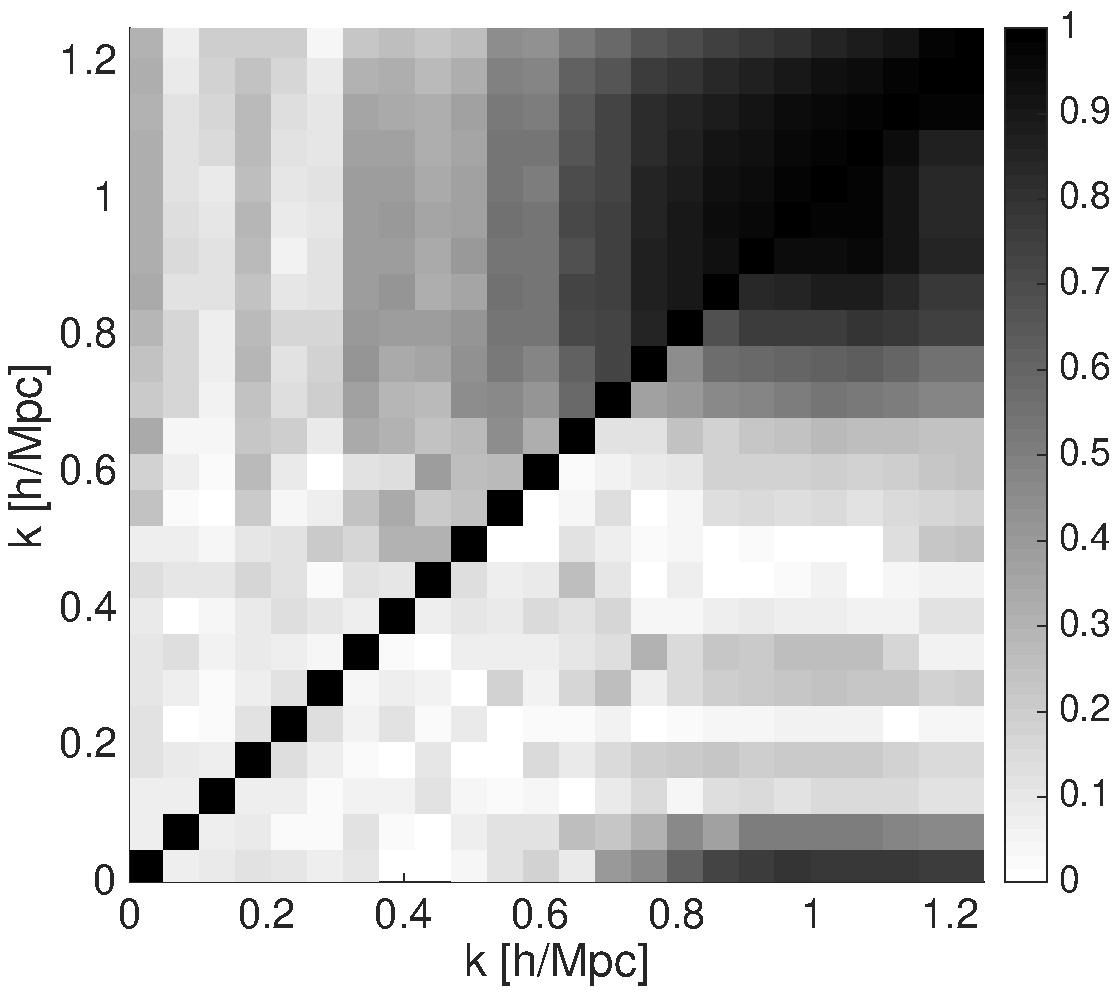
\includegraphics[width=0.48\textwidth]{corr_cut-crop.pdf}
%  \caption{Cross-correlation coefficient matrix as found from 136 power spectra of the non-linear 
%density field from simulation (the upper triangle) and the deformation potential field from 
%reconstruction(the lower triangle).} 
%
%    \label{fig:corrall}
%\end{figure}
    Mathamatically, Fisher information \cite{bib:Tegmark1997} $I$ in the log of amplitude $A$ of the initial 
matter power spectrum is difined as 
\begin{align}
   I \equiv - \langle \frac{\partial ^2 \mathrm{ln \Largr}}{\partial A ^2} \rangle,
\label{eq:fisherdefine}
\end{align}
   in which $\Largr$ denotes the likelihood. For Gaussian fluctuations, the likelihood depends on
parameter only through the power spectrum $P(k)$, and the information $I$ defined by \ref{eq:fisherdefine}
can be written as \cite{bib:Rimes2006}
\begin{align}
    I = - \left\langle \sum_{k,k'} \frac{\partial \mathrm{ln} P(k)}{\partial \mathrm{ln} A} 
\frac{\partial ^2 \mathrm{ln \Largr}}{\partial \mathrm{ln} P(k) \partial \mathrm{ln} P(k')}
\frac{\partial \mathrm{ln} P(k')}{\partial \mathrm{ln} A}\right\rangle
\label{eq:fisherdefineforgaussian}
\end{align}
    For any density field $\delta$, we can conveniently decompose it as
\begin{align}
    \delta (k) = b (k) \delta _L (k) + n (k)
\label{eq:decompose}
\end{align}
in which $\delta_L$ denotes the linear density field. Safely select $b (k)$ and $n (k)$ 
so that the correlation $\langle \delta_l (k) n (k) \rangle$ is zero. Correlating the density field 
$\delta$ and linear density field $\delta_L$,
\begin{align}
   \langle \delta (k) \delta_L (k) \rangle = b (k) \langle \delta_L (k) \delta_L (k) \rangle,
\label{eq:correlating}
\end{align} 
    we obtain
\begin{align}
    b (k) = \frac{P _{\delta \delta_L}(k)}{P_{\delta_L}(k)}.
\label{eq:bofk}
\end{align}
Nonlinear evolution drives $b (k)$ to drop from unity, and generates the noice $n (k)$. 
Correlating the density field $\delta$ and itself, we can write it's power spectrum as
\begin{align}
   P_\delta (k) = \mathcal{D} (k) P_{\delta_L} (k) + P_n (k),
\label{eq:powerdecompose}
\end{align}
where $\mathcal{D} \equiv b^2 (k)$ is the non-liear damping factor, also used in BAO research \tcr{need to cite?}
and $P_n$ is the mode-coupling term.

   With the help of (\ref{eq:bofk}) and (\ref{eq:powerdecompose}), we can replace the partial derivatives 
$\partial \mathrm{ln} p(k) / \partial \mathrm{ln} A$ in (\ref{eq:fisherdefineforgaussian}) to the square of 
cross-correlation $r ^2 (k)$ of $\delta$ and $\delta_L$. the second partial derivative terms in 
\ref{eq:fisherdefineforgaussian}, the Hessian of the vector $\mathrm{ln} P(k)$, has the expectation 
value of the Fisher matrix with respect to the log powers. For linear density fields, the Fisher matrix is 
approximately equal to the inverse of the covariance matrix of power spectrum estimates, which should be diagonal, 
with diagonal elements equal to the number of modes in each wavenumber bin (when considering $\bs{k} and -\bs{k}$ 
as the same mode). We can write down a simpler form of the definition of Fisher information in (\ref{eq:fisherdefineforgaussian}), 
\begin{align}
    I \left( < k_n\right) = r^2(k)^{\mathrm{T}} \left[ \mathrm{C^{-1}_{norm}} \left( k_i,k_j \right)\right] \left( i,j \leq n \right) r^2(k'),
\label{eq:fisherformulaused}
\end{align}
where $\mathrm{C_{norm}}$ is the normalized covariance matrix with size per dimension up to $k_n$, defined as
\begin{align}
    \mathrm{C_{norm}} \left( k,k' \right)=\frac{\mathrm{Cov}(k,k')}{\langle P(k)\rangle\langle P(k)\rangle},
\end{align}
and $r$ is the mean cross-correlation of non-linear, linear and reconstructed density field and linear one up to $k_n$. 
It's reliable to define samely as (\ref{eq:fisherformulaused}) for non-linear density fields, 
since the Fisher matrix is approximately the same as that of linear density fields in linear scale. 
The covariance matrix is defined as 
\begin{align}
    \mathrm{Cov}\left(k,k'\right)\equiv \frac{1}{N-1}\sum_{i=1}^{N}\left[ P_i \left( k \right) - 
\langle P \left( k \right) \rangle \right]\left[ P_j \left( k' \right) - \langle P \left( k' \right)\rangle \right],
\end{align}
where angle brackets mean the expected values.
    The the correlation matrix, is a                                                    
normalized version of the covariance matrix,
\begin{align}
    \mathrm{Corr}\left(k,k'\right)=\frac{\mathrm{Cov}\left(k,k'\right)}{\sqrt{\mathrm{Cov}\left(k,k\right)\mathrm{Cov}\left(k',k'\right)}}.
\end{align}
The corelation matrices for density fields from simulations and deformation potentials from
reconstructions are shown in Fig. \ref{fig:corrall}. For the original density fields, the
linear regime, where $k<0.1$, is diagonal, while in the non-linear regime, the power spectra of
different $k$ modes are strongly correlated by at least $60\%$ . For the reconstructed deformation
potential correlation matrix, however, the linear regime expand up to $k~0.2$. The correlation
matrix is closer to that for the power spectra of linear density fields.
\begin{figure}
 \centering
  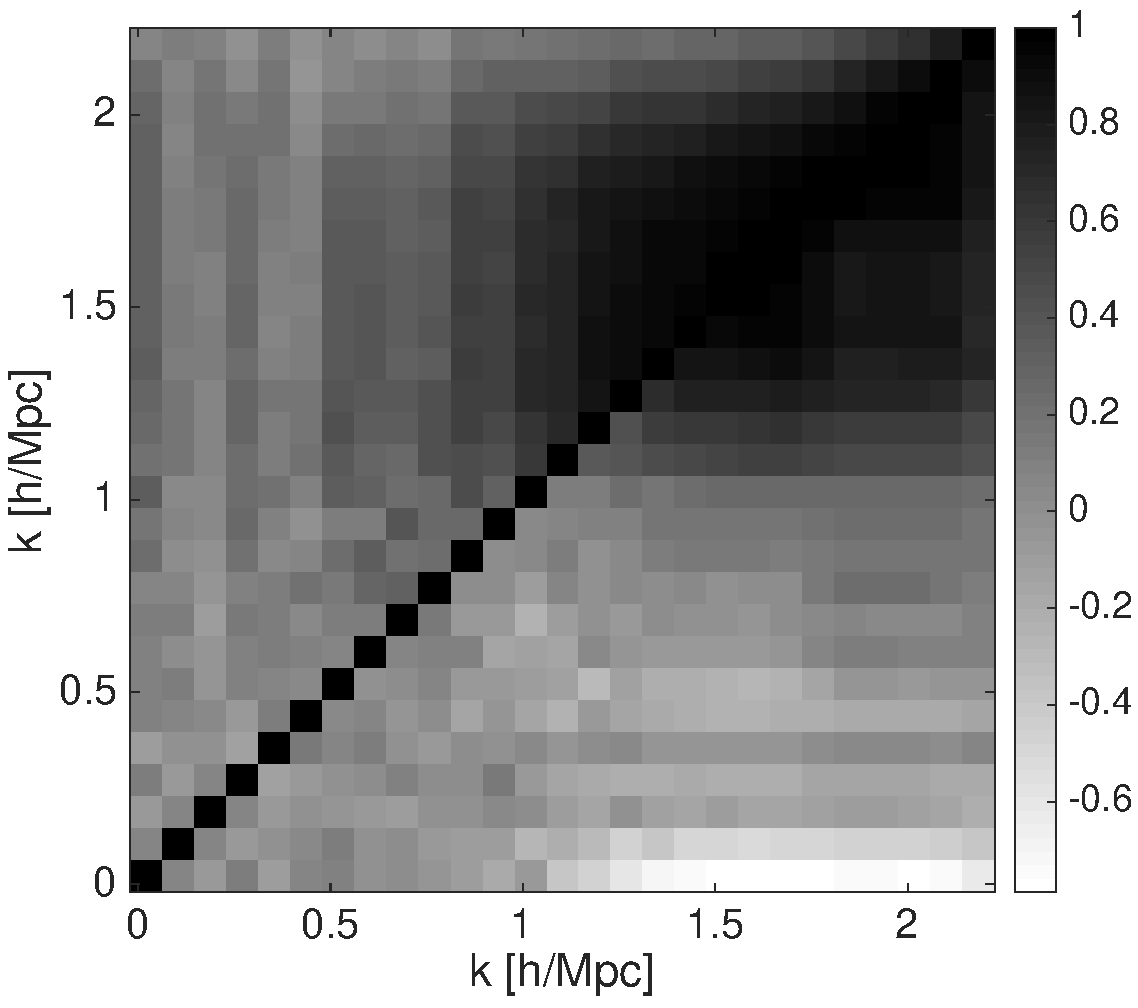
\includegraphics[width=0.48\textwidth]{corrmatrix_good-crop.pdf}
  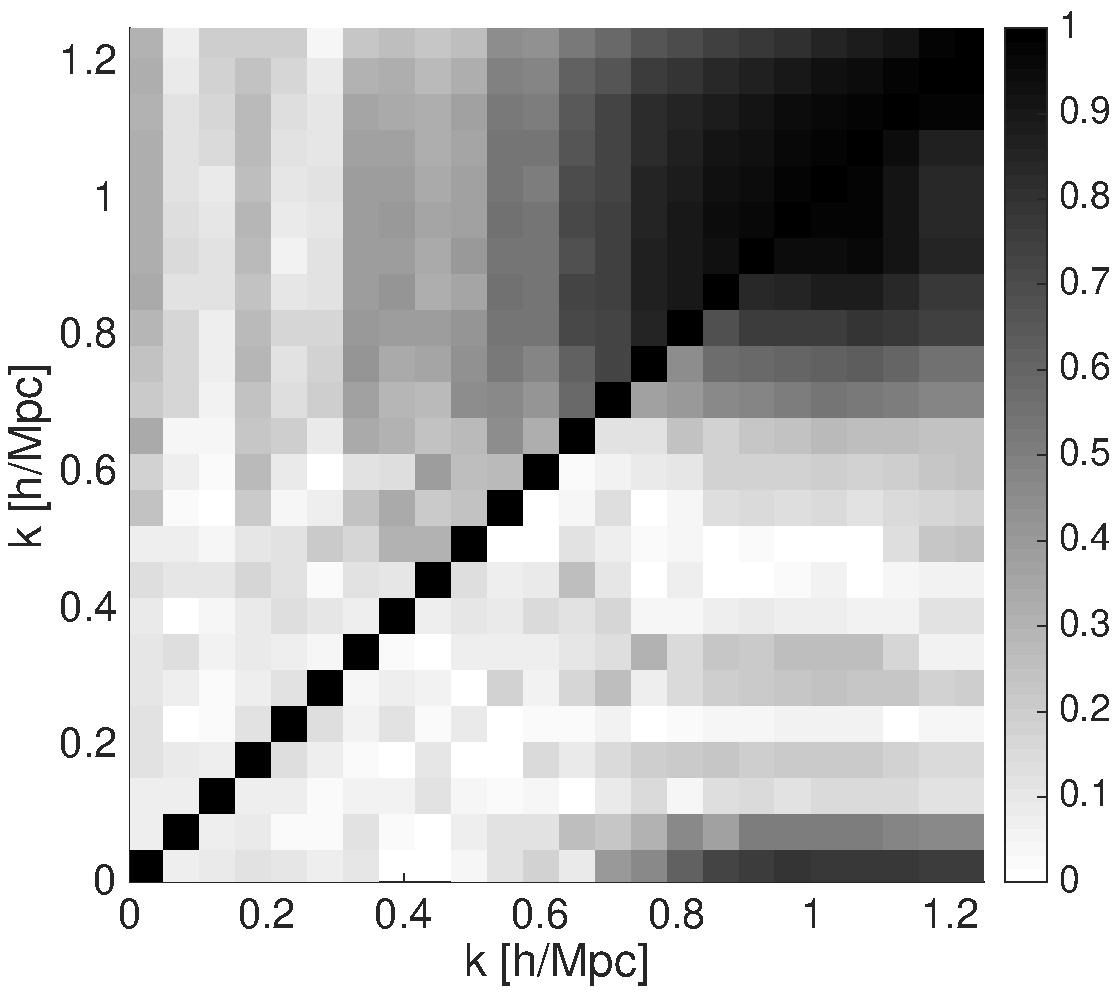
\includegraphics[width=0.48\textwidth]{corr_cut-crop.pdf}
  \caption{Cross-correlation coefficient matrix as found from 136 power spectra of the non-linear
density field from simulation (the upper triangle) and the deformation potential field from
reconstruction(the lower triangle).}

    \label{fig:corrall}
\end{figure}

%  The signal-to-noise ratio, sometimes also called Fisher information, can be given by the inverse matrix of covariance. Since the signal-to-noise ratio was given in some work, we also present it for a better comparison. 
%\begin{align}
%\left( \frac{S}{N}\right)^2 (k_{n}) =\sum_{i,j=1}^n P_i \mathrm{Cov}^{-1}(i,j) P_j
%\end{align}

  As seen above, cumulative information is a measurement of the number of independent Fourier modes 
presented in a field up to a given $k_n$, which represents how linear a field is. We plot the 
cumulative information of the power specta of density fields from simulations and deformation 
potentials from reconstructions in Fig.\ref{fig:fisherinfo}. In the translinear regime, where 
$k\sim0.1$, the cumulative information of the non-linear density field has a flat plateau. It 
indicates that there's nearly no independent information in the translinear regime of the power 
spectrum. At $k\sim0.8$, the information increase slightly aggain. But the information curve of 
the reconstructed deformation potential keeps incresing and reaches it's plateau at $k\sim0.6-0.7$ 
up to a factor of 20. It indicates that APM method can strongly recover the lost information within this scale. 
\begin{figure}[t!]
%[htbp]
 \begin{center}
  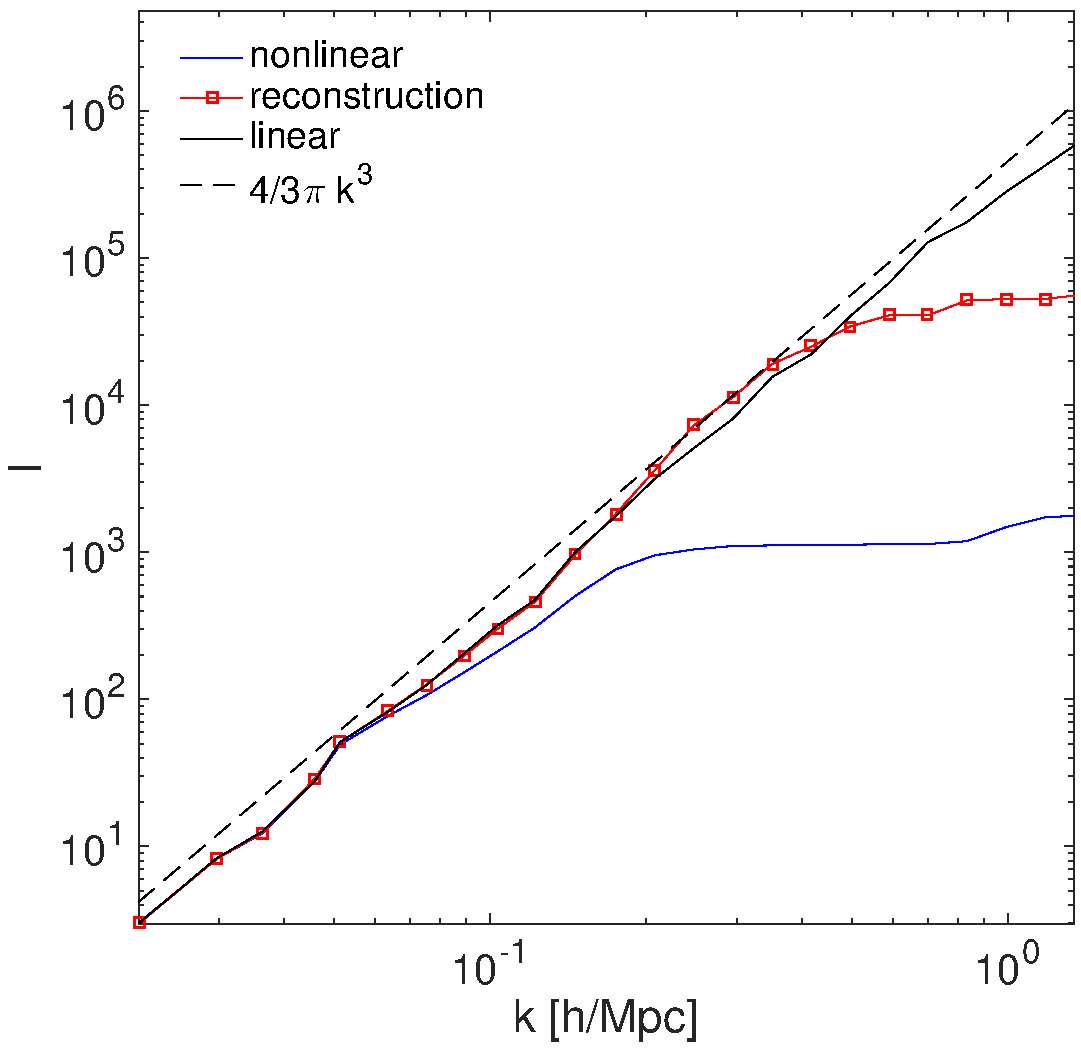
\includegraphics[width=0.48\textwidth]{fisher_1-crop.pdf}
  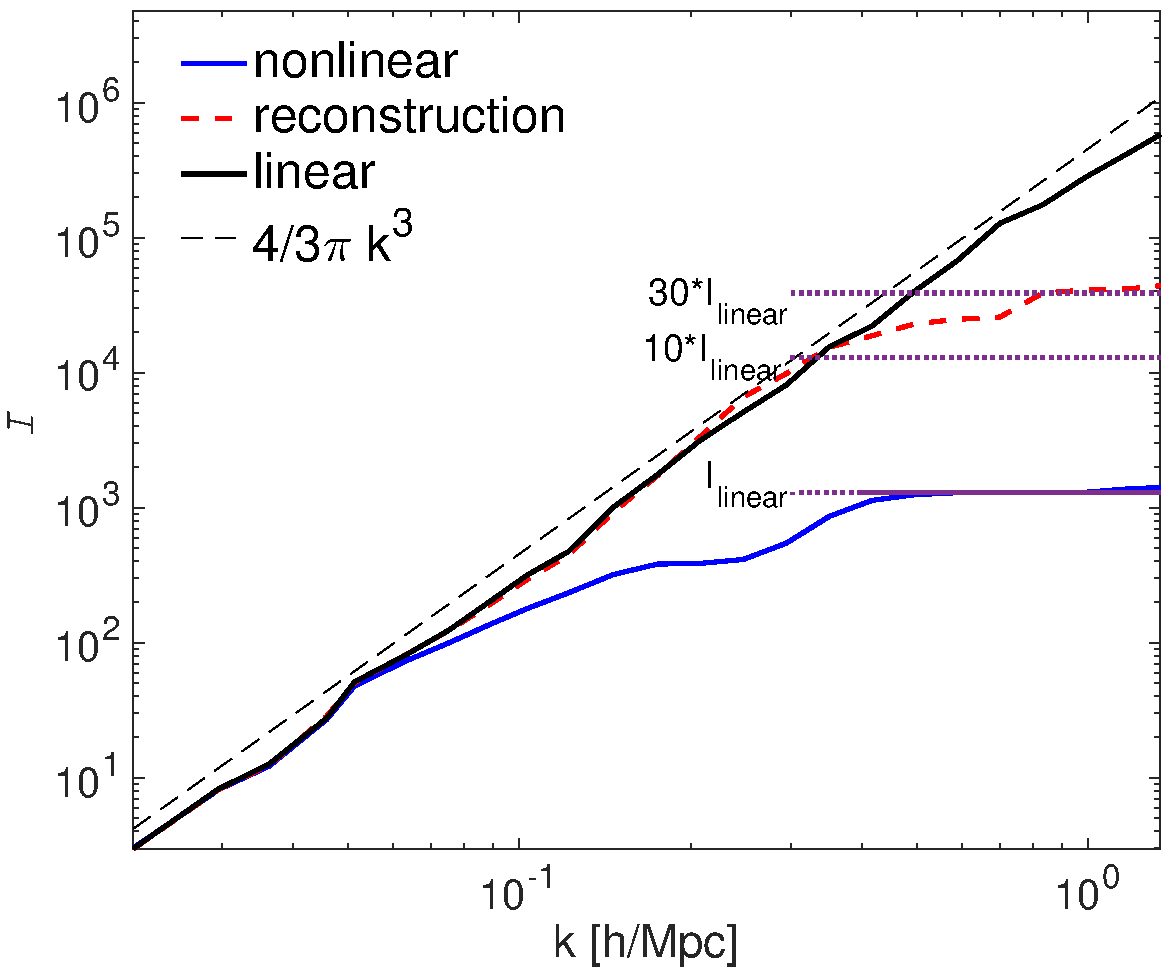
\includegraphics[width=0.48\textwidth]{fisher_full-crop.pdf}
  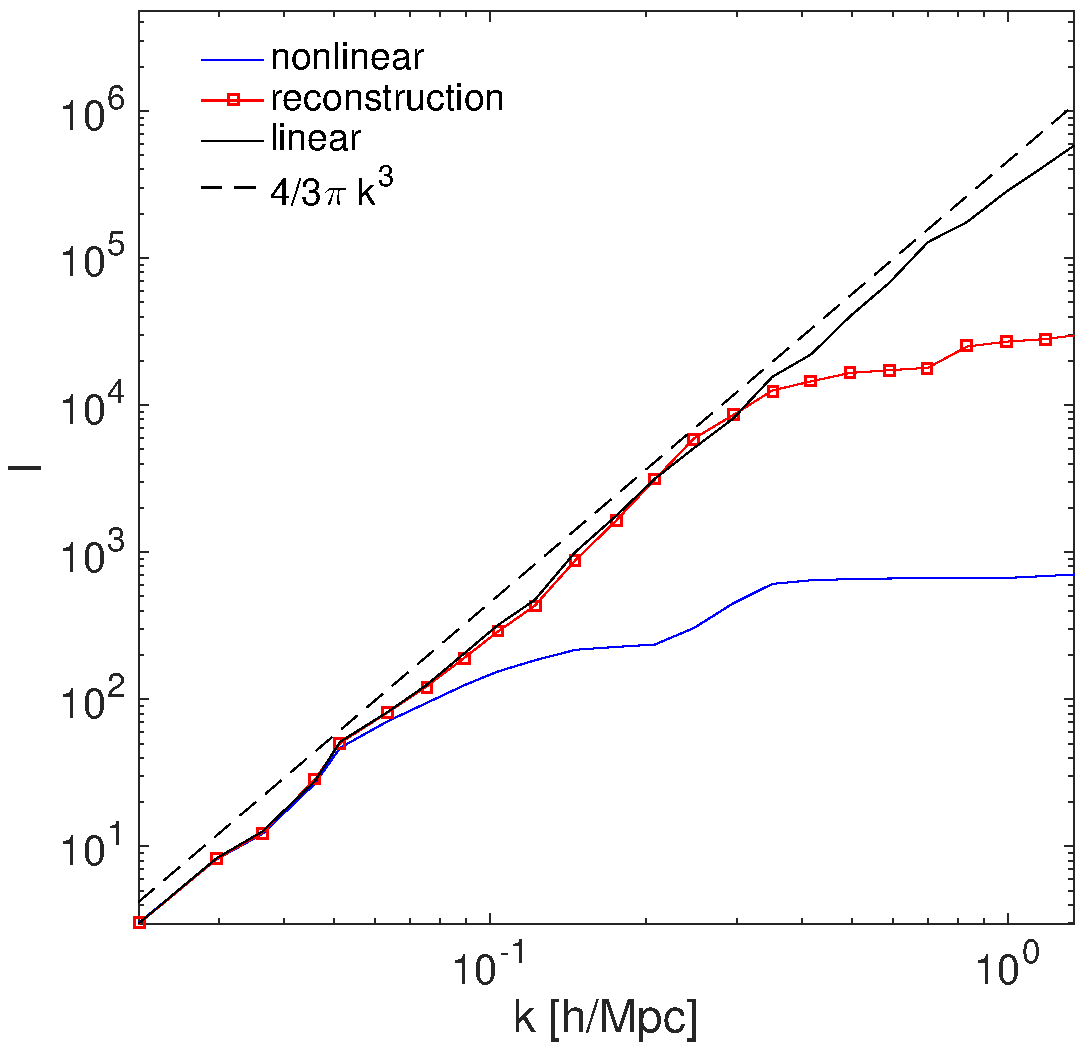
\includegraphics[width=0.48\textwidth]{fisher_r2-crop.pdf}
%  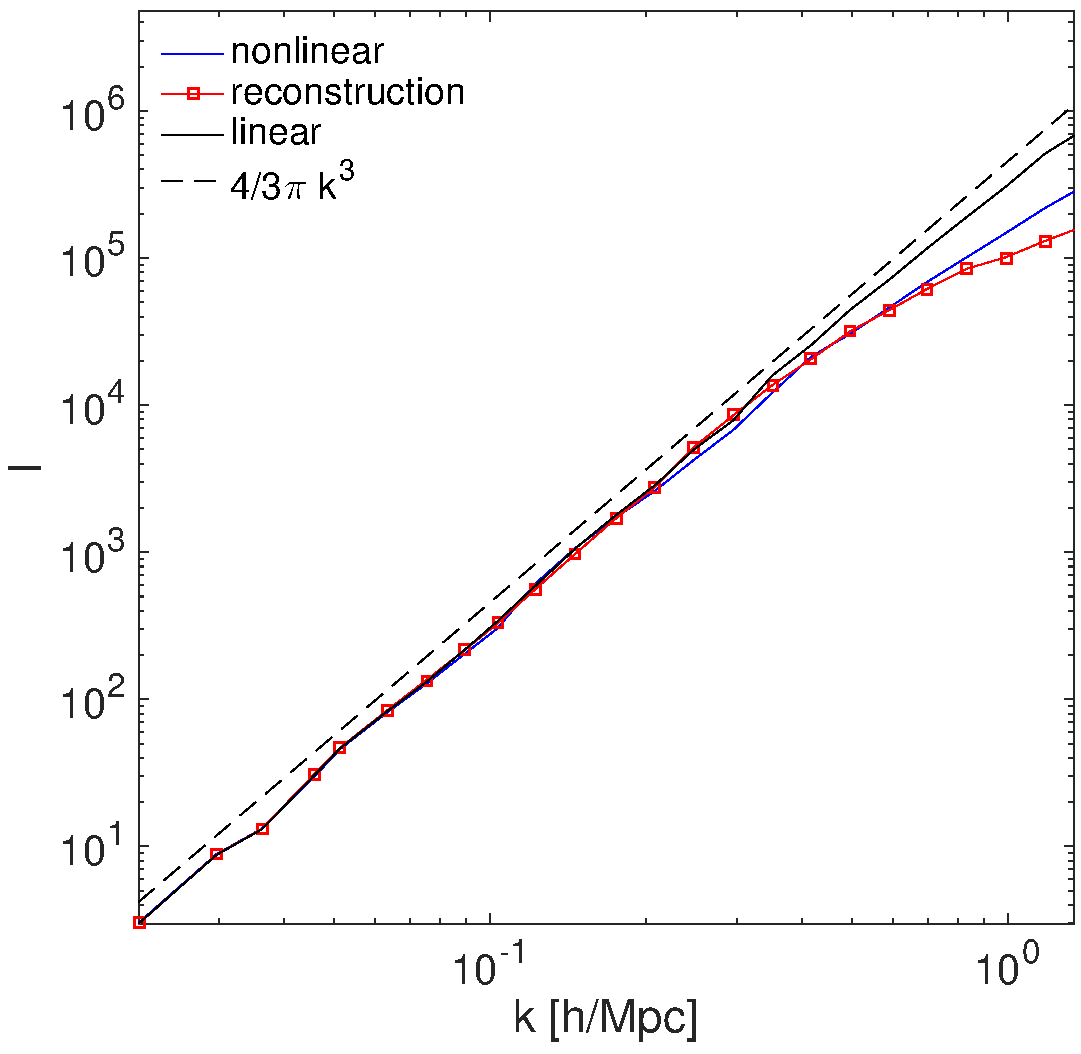
\includegraphics[width=0.48\textwidth]{fisher_tr-crop.pdf}
%  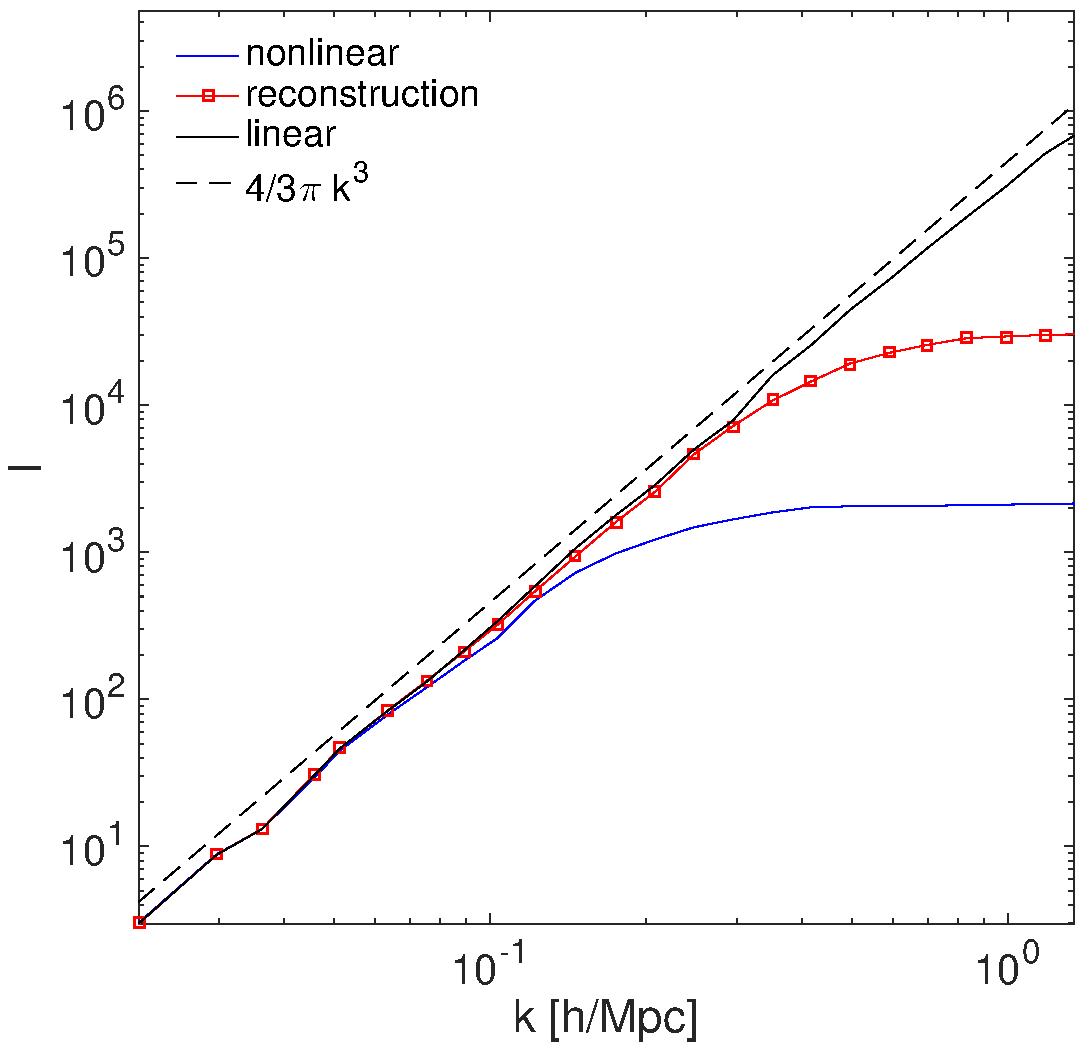
\includegraphics[width=0.48\textwidth]{fisher_trr2-crop.pdf}
   \caption{Cumulative information in the power spectra as a function of wavenumber. The blue 
cycles correspond to the non-linear density field by simulation; the black squares correspond 
to the the reconstructed deformation potential; the red dash line corresponds to linear density 
field at $z=0$; the green crosses correspond to linear density field at $z=100$.}
  \label{fig:fisherinfo}
 \end{center}
\end{figure}
\begin{figure}[t!]
\centering
  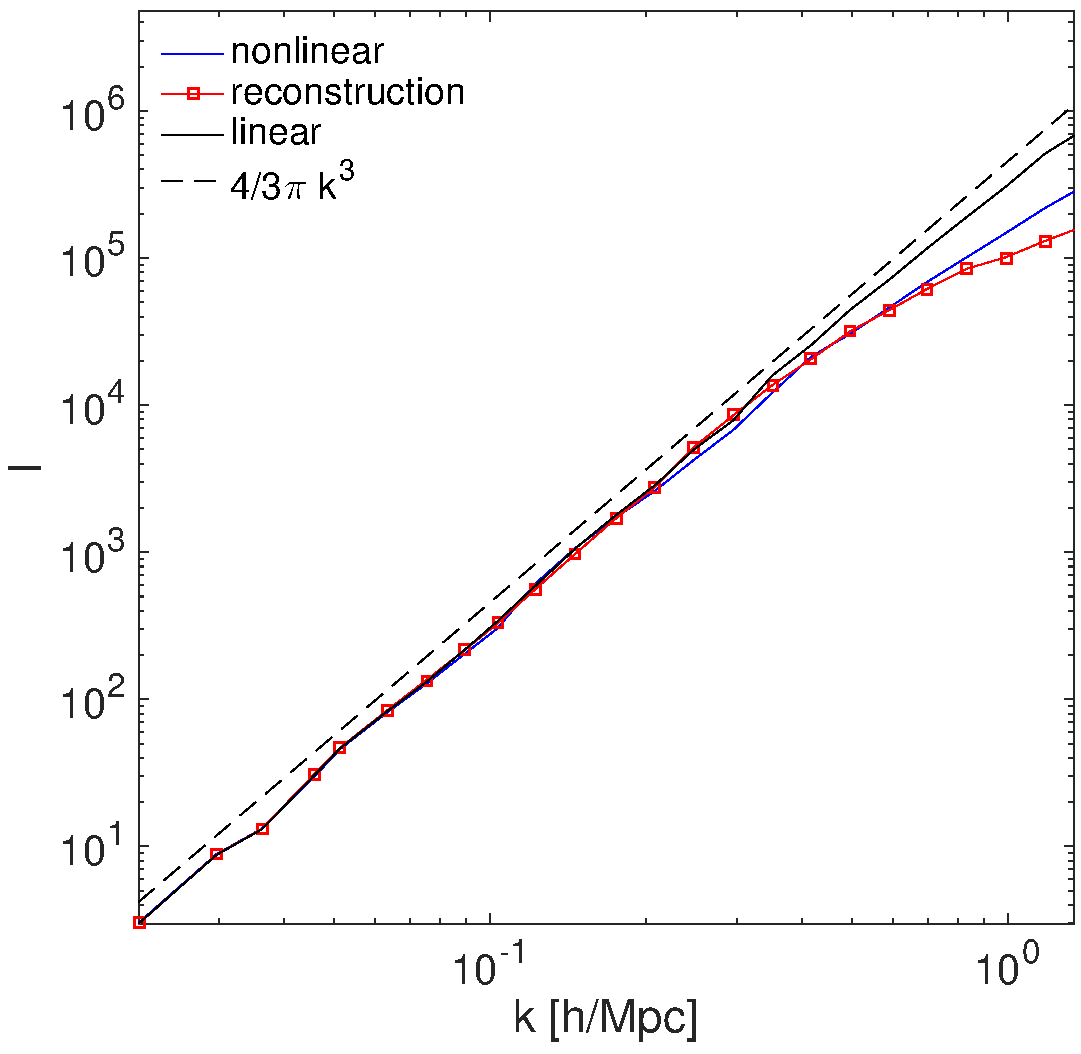
\includegraphics[width=0.48\textwidth]{fisher_tr-crop.pdf}
  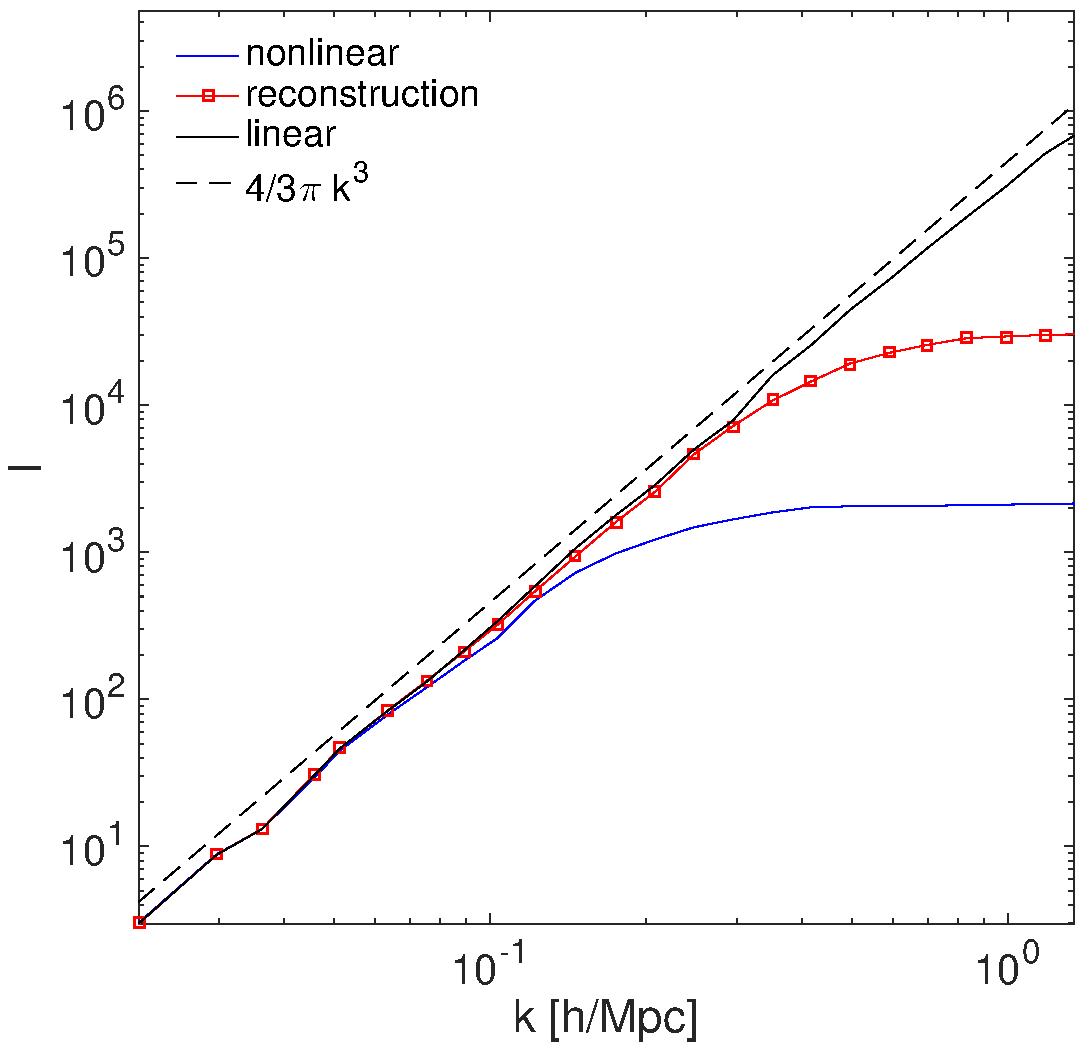
\includegraphics[width=0.48\textwidth]{fisher_trr2-crop.pdf}
\end{figure}

\end{section}
